\section{Models}
\label{sec:models}
Three different categories of models were
considered:
\begin{itemize}
    \item \textit{Decision Trees}
    \item \textit{Random Forests}
    \item \textit{Neural Networks}
    \begin{itemize}
        \item \textit{Feedforward Networks}
        \item \textit{LSTM Networks}
    \end{itemize}
\end{itemize}
Decision Trees and Random Forests both use
the BoW preprocessing with \textbf{binary} 
encoding.
Feedforward Neural Networks use the BoW
preprocessing with \textbf{TFIDF} encoding.
LSTM Networks were tested with both the
WE and GE preprocessing.

\subsection{Imbalanced Dataset}
To handle the imbalanced dataset, a class
weight was assigned to each class. The weight
for a class $c$ was calculated as
$W_c=\frac{|D|}{|C||D_c|}$ where $|D|$ is
the size of the dataset, $|C|$ is the number
of classes and $|D_c|$ is the number of
samples in class $c$. This weight was used in
the criterion of the Decision Trees and Random
Forests models, and in the loss function of
the Neural Networks models.

\subsection{Model Selection}
To find a good hyperparameter configuration
for each model, a random search was performed.
The search was done with 10 iterations for
each model (Decision Trees, Random Forests 
and Neural Networks). Each configuration was
evaluated with a 6-fold cross-validation on
the training set. Two subsequent random
searches were performed, the second one
narrowing the search space around the best
configuration found in the first search.
The search spaces for each model are shown
in \autoref{tab:dt_search_spaces_1}, 
\autoref{tab:rf_search_spaces_1} and 
\autoref{tab:nn_search_spaces_1} for the 
first search, and in 
\autoref{tab:dt_search_spaces_2},
\autoref{tab:rf_search_spaces_2} and
\autoref{tab:nn_search_spaces_2} for the
second search.

\begin{table}[H]
\centering
\begin{tabularx}{0.48\textwidth}{|l|X|}
\hline
Hyperparameter & Search Space \\
\hline
\texttt{criterion} & \{gini, entropy, log\_loss\} \\
\texttt{splitter} & \{best\} \\
\texttt{max\_depth} & \{10, 100, None\} \\
\texttt{min\_impurity\_decrease} & \{0.01, 0.0001, 1e-06, 1e-08, 0\} \\
\texttt{class\_weight} & \{balanced\} \\
\hline
\end{tabularx}
\caption{Decision Trees hyperparameter search space for the first search.}
\label{tab:hyperparameters_decision_tree_0}

\end{table}


\begin{table}[H]
\centering
\begin{tabularx}{0.48\textwidth}{|l|X|}
\hline
Hyperparameter & Search Space \\
\hline
\texttt{n\_estimators} & \{10, 50, 100\} \\
\texttt{criterion} & \{gini, entropy, log\_loss\} \\
\texttt{max\_depth} & \{10, 100, None\} \\
\texttt{min\_impurity\_decrease} & \{0.01, 0.0001, 1e-06, 0\} \\
\texttt{n\_jobs} & \{-1\} \\
\texttt{class\_weight} & \{balanced\} \\
\hline
\end{tabularx}
\caption{Random Forest hyperparameter search space for the first search.}
\label{tab:hyperparameters_random_forest_0}

\end{table}


\begin{table}[H]
\centering
\begin{tabularx}{0.48\textwidth}{|l|X|}
\hline
Hyperparameter & Search Space \\
\hline
\texttt{network} & \{ff\_tfidf, lstm\_embeddings\} \\
\texttt{base\_size} & \{8, 16, 32\} \\
\texttt{depth} & \{1, 2, 3, 4\} \\
\texttt{epochs} & \{10, 15\} \\
\texttt{dropout} & \{0.5\} \\
\texttt{batchnorm} & \{True, False\} \\
\texttt{batch\_size} & \{32\} \\
\texttt{lr} & \{0.01, 0.001\} \\
\texttt{optimizer} & \{adam\} \\
\hline
\end{tabularx}
\caption{Neural Networks hyperparameter search space for the first search. While using the \texttt{ff\_tfidf} network, if \texttt{batchnorm} is set to \texttt{True}, the \texttt{dropout} hyperparameter is set to $0$. When using the \texttt{lstm\_embeddings} and \texttt{lstm\_glove} networks, the \texttt{batchnorm} hyperparameter is set to \texttt{False}.}
\label{tab:hyperparameters_neural_network_0}

\end{table}


\begin{table}[H]
\centering
\begin{tabularx}{0.48\textwidth}{|l|X|}
\hline
Hyperparameter & Search Space \\
\hline
\texttt{criterion} & \{gini, log\_loss\} \\
\texttt{splitter} & \{best\} \\
\texttt{max\_depth} & \{1000, None\} \\
\texttt{min\_impurity\_decrease} & \{1e-05, 1e-06, 1e-07\} \\
\texttt{class\_weight} & \{balanced\} \\
\hline
\end{tabularx}
\caption{Decision Trees hyperparameter search space for the second search.}
\label{tab:hyperparameters_decision_tree_1}

\end{table}


\begin{table}[H]
\centering
\begin{tabularx}{0.48\textwidth}{|l|X|}
\hline
Hyperparameter & Search Space \\
\hline
\texttt{n\_estimators} & \{100, 125, 150\} \\
\texttt{criterion} & \{gini, log\_loss\} \\
\texttt{max\_depth} & \{1000, None\} \\
\texttt{min\_impurity\_decrease} & \{1e-05, 1e-06, 1e-07\} \\
\texttt{n\_jobs} & \{-1\} \\
\texttt{class\_weight} & \{balanced\} \\
\hline
\end{tabularx}
\caption{Random Forest hyperparameter search space for the second search.}
\label{tab:hyperparameters_random_forest_1}

\end{table}


\begin{table}[H]
\centering
\begin{tabularx}{0.48\textwidth}{|l|X|}
\hline
Hyperparameter & Search Space \\
\hline
\texttt{network} & \{ff\_tfidf, lstm\_glove\} \\
\texttt{base\_size} & \{16, 32\} \\
\texttt{depth} & \{1, 2, 3\} \\
\texttt{epochs} & \{20\} \\
\texttt{patience} & \{2\} \\
\texttt{dropout} & \{0.5\} \\
\texttt{batchnorm} & \{False\} \\
\texttt{batch\_size} & \{32\} \\
\texttt{lr} & \{0.001\} \\
\texttt{optimizer} & \{adam\} \\
\hline
\end{tabularx}
\caption{Neural Networks hyperparameter search space for the second search. The same rules described in \autoref{tab:hyperparameters_neural_network_0} apply.}
\label{tab:hyperparameters_neural_network_1}

\end{table}




Accuracy was used as the metric to evaluate
the models and we can see the results in
\autoref{fig:model_selection}.

\end{multicols}
\begin{figure}[H]
    \centering
    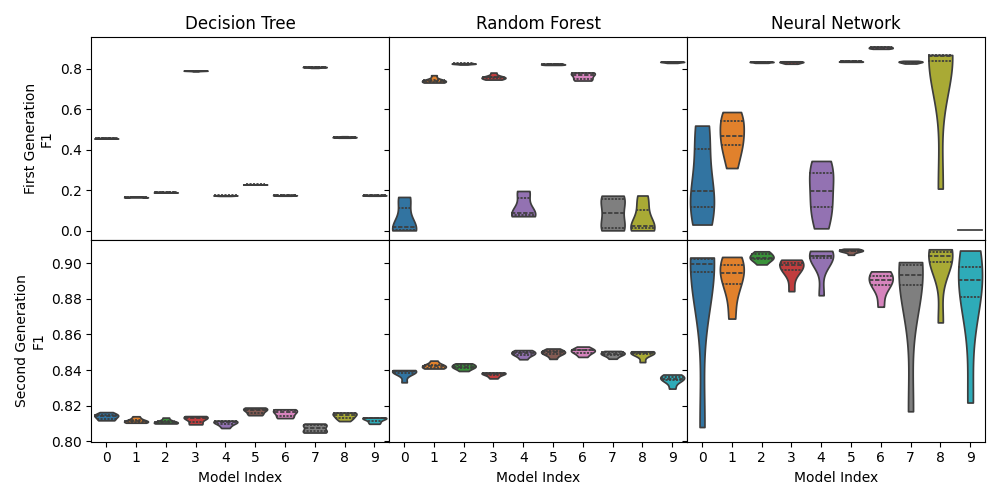
\includegraphics[width=\textwidth]{images/model_selection.png}
    \caption{Accuracy distribution of each model configuration tested during the model selection process.}
    \label{fig:model_selection}
\end{figure}

\begin{figure}[H]
    \centering
    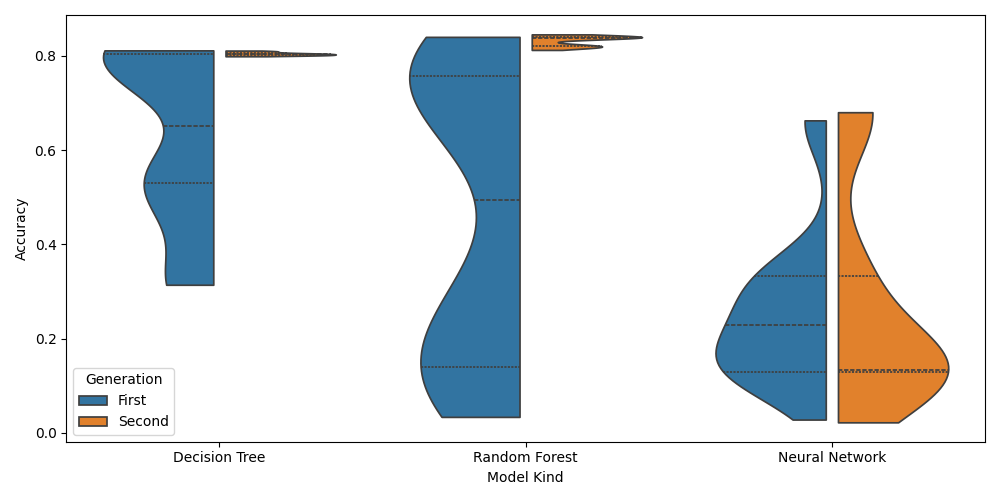
\includegraphics[width=\textwidth]{images/accuracy_distribution.png}
    \caption{Accuracy distribution of each model category.}
    \label{fig:accuracy_distribution}
\end{figure}
\begin{multicols}{2}

The best model was selected based on 
the average accuracy obtained in the
cross-validation. The accuracy distribution
of this model was compared to the other
models with a Wilcoxon signed-rank test,
some models were not significantly different 
($p>0.05$) from the best model and they 
are listed in \autoref{tab:best_models}.

\begin{table}[H]
    \centering
    \begin{tabular}{|l|r|}
        \hline
        \textbf{Model ID} & \textbf{Average Accuracy} \\
        \hline
        \texttt{neural\_network-G1-0} & $82.00\%$ \\
        \hline
    \end{tabular}
    \caption{Best model (first row) and models not significantly different from the best model.}
    \label{tab:best_models}
\end{table}